% Created 2019-07-15 Mon 21:59
% Intended LaTeX compiler: pdflatex
\documentclass[11pt]{article}
\usepackage[utf8]{inputenc}
\usepackage[T1]{fontenc}
\usepackage{graphicx}
\usepackage{grffile}
\usepackage{longtable}
\usepackage{wrapfig}
\usepackage{rotating}
\usepackage[normalem]{ulem}
\usepackage{amsmath}
\usepackage{textcomp}
\usepackage{amssymb}
\usepackage{capt-of}
\usepackage{hyperref}
\usepackage[margin=2cm]{geometry}
\usepackage{pdfpages}
\author{Josh (W0ODJ), Ken (KM4NFQ)}
\date{\today}
\title{K5BCQ K3NG Keyer v0.6}
\hypersetup{
 pdfauthor={Josh (W0ODJ), Ken (KM4NFQ)},
 pdftitle={K5BCQ K3NG Keyer v0.6},
 pdfkeywords={},
 pdfsubject={},
 pdfcreator={Emacs 26.1 (Org mode 9.2.3)}, 
 pdflang={English}}
\begin{document}

\maketitle
\tableofcontents


\section{Introduction}
\label{sec:org8efcbbc}
This keyer is a design of the proposed schematic provided by Anthony Good (K3NG) on his website, \href{https://blog.radioartisan.com/arduino-cw-keyer}{Radioartisan}.  As taken from his website:
\begin{quote}
"This is an open source Arduino based CW (Morse Code) keyer with a lot of features and flexibility, rivaling commercial keyers which often cost significantly more.  The code can be used with a full blown Arduino board or an AVR microcontroller chip can be programmed and used directly in a circuit.  This keyer is suitable as a standalone keyer or for use permanently installed inside a rig, especially homebrew QRP rigs.  It’s open source code so you can fully customize it to fit your needs and also perhaps learn from it or find coding ideas for other projects."
\end{quote}


This board is an attempt to provide an outline for utilizing many of the options available in Goody's amazing open-source arduino-based morse code keyer.  Mechanisms are available for multiple size LCDs, I2C displays, 2 transmitter outputs, a Goertzel audio decoding input, rotary encoder for speed control, seven memories, hookups for both 3x4 and 4x4 number pads, amongst others.  It is designed to be built for only the modules you need - you do not need to populate those you are not going to use!

This documentation is specific for the K5BCQ board of the K3NG keyer.  However, in most locations you can change the hardware specific reference (e.g. \emph{"keyer\_pin\_settings\_k5bcq.h"} to the generic reference \emph{"keyer\_pin\_settings.h"}) relatively easily.  That means the comments regarding pinouts, enabling features, etc - should all be mostly universal (though specific pins, etc. will likely change).

The PCB images of part locations have been painstakingly created by Ken, KM4NFQ.  He has graciously allowed them to be included in this documentation.

\section{Bill of Materials}
\label{sec:orgd9a9a71}
\begin{center}
\begin{tabular}{llrll}
\textbf{Reference} & \textbf{Value} & \textbf{Quantity} & \textbf{Digikey \#} & \textbf{Notes}\\
\hline
R1, 2, 3, 4, 5, 6, 7 & 1k & 7 & CF18JT1K00CT-ND & 1/8w\\
R12, 18, 27, 28 & 1k & 4 & CF14JT1K00CT-ND & 1/4w\\
R16, 17, 21, 22 & 10k & 5 & CF14JT10K0CT-ND & 1/4w\\
R9 & 10k & 1 & CF18JT10K0CT-ND & 1/8w\\
R15 & 220 & 1 & CF18JT220RCT-ND & 1/8w\\
R13, 19, 20, 26 & 220 & 4 & CF14JT220RCT-ND & 1/4w\\
R14, 23, 36 & 100 & 3 & CF14JT100RCT-ND & 1/4w\\
R24, 25 & 4.7k & 2 & CF14JT4K70CT-ND & 1/4w\\
R30, 31, 33 & 3.3k & 3 & CF18JT3K30CT-ND & 1/8w\\
R32 & 560 & 1 & CF18JT560RCT-ND & 1/8w\\
R34 & 10 & 1 & CF18JT10R0CT-ND & 1/8w\\
R35 & 150k & 1 & CF18JT150KCT-ND & 1/8w\\
R37 & 100k & 1 & CF18JT100KCT-ND & 1/8w\\
R8, 11, 29 & 20k & 3 & 3306F-203-ND & 6mm top-adjust trimpot\\
R10 & 500 & 1 & 3306F-501-ND & 6mm top-adjust trimpot\\
C1, 2, 3, 5, 7, 8 & 10nF & 6 & 490-8634-ND & \\
C6, 9, 10, 11a, 11b, 12, 13 & 100nF & 7 & 445-173396-1-ND & \\
C4 & 100uF & 1 & 493-6095-1-ND & Electrolytic\\
C14, 15, 16, 17 & 10uF & 4 & P19580CT-ND & Electrolytic\\
Q1, 3, 4, 6, 8 & 2N7000 & 5 & 2N7000FS-ND & TO-92\\
Q2, 5, 7 & 2N3904 & 3 & 2N3904FS-ND & TO-92\\
LED1, 2, 3, 4 &  & 4 &  & LED of your choice of colors\\
SW1 &  & 1 & 987-1398-ND & Rotary encoder with switch\\
SW2, 3, 4, 5, 6, 7, 8 &  & 7 & 450-1642-ND & 6mm x 6mm NO tactile switch\\
J1, 2, 3, 4, 5 &  & 5 & SC1461-ND & PJ-325M, \href{https://www.digikey.com/product-detail/en/switchcraft-inc/35RAPC4BV4/SC1461-ND/528670}{These} should work\\
J6 &  & 1 & CP-002A-ND & DC plug\\
X1 &  & 1 & CP-2260-ND & MiniDin 6 - \href{https://www.digikey.com/product-detail/en/cui-inc/MD-60SM/CP-2260-ND/96940}{MD-60SM}\\
SP1 &  & 1 &  & Off-board speaker\\
U1 & Display & 1 &  & 1602, 1604, 2004 Serial LCD\\
U2 & Mega2560 & 1 &  & Mini variant, \href{https://robotdyn.com/mega-2560-pro-mini-atmega2560-16au.html}{here}\\
U3 & Keypad & 1 &  & 3x3 or 3x4 keypad\\
P1, 2, 4A, 4P, ASR-JP &  &  &  & 2.54mm Male headers\\
\end{tabular}
\end{center}
\textbf{*} Part footprints should be correct - BUT I HAVE NOT CONFIRMED!!! Particularly capacitors lead spacing!***


\subsection{Which Arduino?}
\label{sec:org5246890}

Of significant importance in the fact that while Arduino(s) is/are "standard," there is great leeway and interpretation in the particular details regarding "standard."  When building the K5BCQ PCB of the K3NG keyer, you must make sure you are purchasing one of the boards with the correct footprint for the PCB.  While many producer's versions (may) work, there is no guarantee.  Just be sure to obtain one with the correct voltage (5v), USB (if desired), and footprint.  Linked above is a known good brand (RobotDyn) for the designed PCB.

\subsubsection{The \textbf{correct} footprint looks like:}
\label{sec:orge5aad90}
\begin{center}
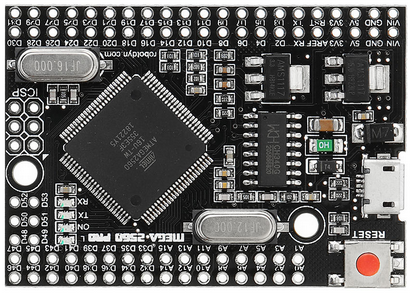
\includegraphics[width=.9\linewidth]{../png/2.1/Correct2560.png}
\end{center}

\subsubsection{The \textbf{incorrect} footprint looks like:}
\label{sec:org0f14868}
\begin{center}
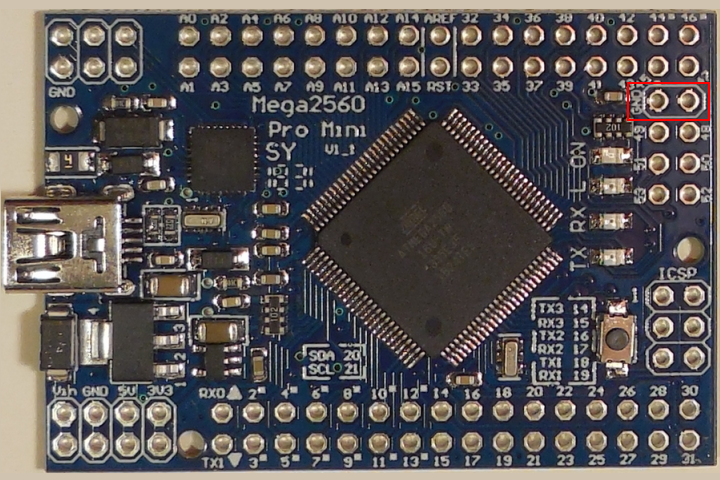
\includegraphics[width=.9\linewidth]{../png/2.1/Wrong2560.png}
\end{center}

The wrong pinout will \emph{still} work, \emph{technically} - but would require manually running jumper wires between the boards, instead of using headers for installation.

\newpage
\section{Build Instructions}
\label{sec:org37f6a82}
Building is relatively straightforward.  Instructions to build all available options is included in the documentation.  If there is a module you do not wish to include, just skip that step.  If there is an issue skipping the step, it will be noted in the documentation for that step.

If you are going to build all of the modules - ignore the following steps.  Just build it normally - lowest parts first.  My preferred order is resistors, capacitors, transistors, headers, buttons and other hardware.

\subsection{Arduino}
\label{sec:org8543ede}
\begin{itemize}
\item[{$\square$}] Arduino
\begin{itemize}
\item[{$\square$}] Arduino Mega 2560 Pro Mini
\item[{$\square$}] 2.54mm Male Headers (1 - 2x21, 1 - 2x16, 1 - 2x3)
\item[{$\square$}] 2.54mm Female Headers (1 - 2x21, 1 - 2x16, 1 - 2x3)
\end{itemize}

The Arduino is installed on the underside of the board.  If you wish, you could directly solder the board to the main PCB using just the male headers - most people prefer the ability to remove the Arduino, however.  It may be easier to install the Arduino and headers AFTER all of the other parts have been installed.  Builder's discretion.

The easiest way to properly, neatly solder the board and headers, is to not solder any of it to begin with.  After cutting/breaking/obtaining the right width and length of headers, start by placing the female headers on the underside of the board.  Once they are in place, NOT SOLDERED, gently place the long portion of the male headers into them.  Not all the way down - just into them.  Once these are in place, then carefully align the male headers into the top of the Mega 2560.  Once they are all in place, squeeze together.  You now will have all of the pins in the correct placement, and they should all be almost perpendicular to the PCBs.  Solder the pins at each end, adjust to make sure they are straight and flush to the PCBs, and then solder the remaining in-between pins.

Once all of the pins are soldered, remove the Arduino and set aside.  You don't want to accidentally short it out.  

\emph{Builder's Note:  You can use single row headers (male and female) instead.  Just be sure to carefully cut and align them, as well as ensure proper fit.  Dual-row headers are preferred for easier mating / removal, but many individuals just use the single row headers side-by-side.}
\end{itemize}
\begin{center}
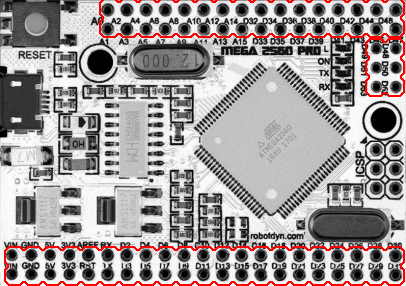
\includegraphics[width=.9\linewidth]{../png/3.1/mega2560-top-headers.png}
\end{center}
\begin{center}
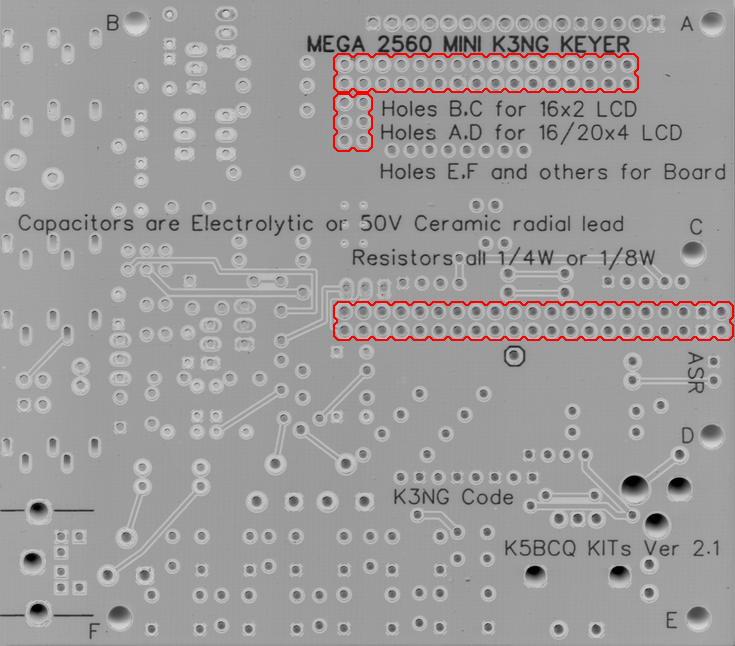
\includegraphics[width=.9\linewidth]{../png/3.1/pcb-bot-mega2560-headers.png}
\end{center}
\newpage
\subsection{Inputs}
\label{sec:orgb482c53}
\begin{itemize}
\item[{$\square$}] Paddle Input
\begin{itemize}
\item[{$\square$}] R16, 17 - 10k\(\Omega\) - (Brown-Black-Orange)
\item[{$\square$}] C1, 2 - 10nF - (103)
\item[{$\square$}] JX - 3.5mm TRS audio jack
\end{itemize}

Input for dual lever paddles.  Designed for the relatively standard 3.5mm TRS (Stereo) jack.  Default wiring is Tip = Dit, Ring = Dah, Sleeve = Ground.  Paddle wiring can be artificaly reversed in software using \texttt{"N"} in command mode (and \texttt{"\textbackslash{}N"} in command line interface).  Using the TRS jack is superior to Mono - it allows both paddle input, as well as Straight Key input.  If you are \uline{only} going to use Straight Key mode, enable \emph{"\#define FEATURE\_STRAIGHT\_KEY"} in \emph{"keyer\_features\_and\_options\_k5bcq.h".}  Paddle pins are set using \emph{"\#define paddle\_left"} and \emph{"\#define paddle\_right"} in \emph{"keyer\_pin\_settings\_k5bcq.h".}

 It is preferred however, to ignore the Straight key functionality (leaving the module disabled), as having it enabled can cause timing / keying issues when using paddles.  Without the module enabled, if you boot the keyer with a properly wired straight key (or a paddle with one key grounded), the keyer will function in straight key mode.  All the benefit, none of the problems!  (unless you \emph{really} need to switch between paddles and straight key that quickly)
\begin{center}
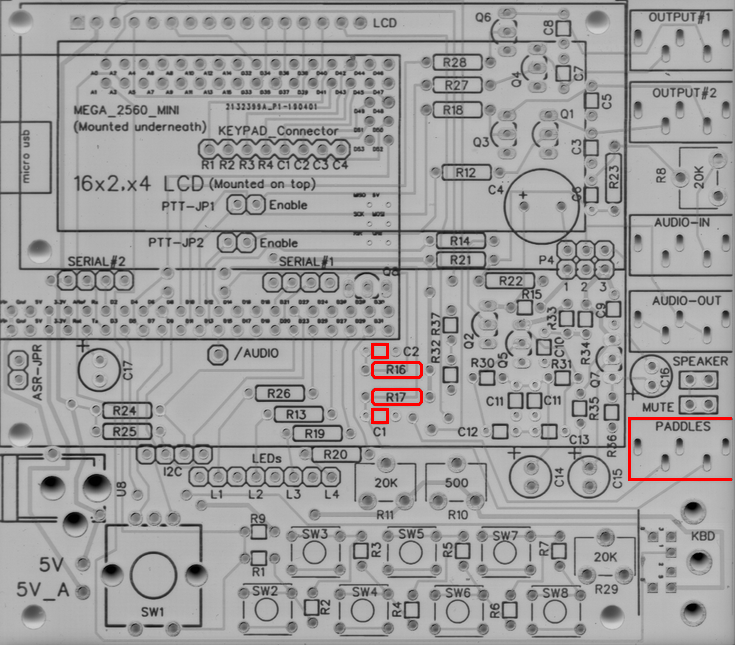
\includegraphics[width=.9\linewidth]{../png/3.2/pcb-top-paddles.png}
\end{center}
\end{itemize}

\newpage
\begin{itemize}
\item[{$\square$}] Memory Buttons
\begin{itemize}
\item[{$\square$}] R1, 2, 3, 4, 5, 6, 7 - 1k\(\Omega\) - (Brown-Black-Red)
\item[{$\square$}] R9 - 10k\(\Omega\) - (Brown-Black-Orange)
\item[{$\square$}] SW2, 3, 4, 5, 6, 7, 8 - 6mm x 6mm NO Tactile push buttons
\end{itemize}
These buttons allow up to seven memories to be utilized.  If you choose not to install them all, you need to edit \emph{"FEATURE\_COMMAND\_BUTTONS"} in \emph{"keyer\_settings\_k5bcq.h"} to accurately represent the number of buttons and the voltage divider used (r1 = R9, r2 = R1-7)

 The height of the tactile button varies wildly based on your intended enclosure.  You may wish to off-board them with wires or headers depending on your design / intention.  For reference, the bottom two mounting holes of each button are ground.
\begin{center}
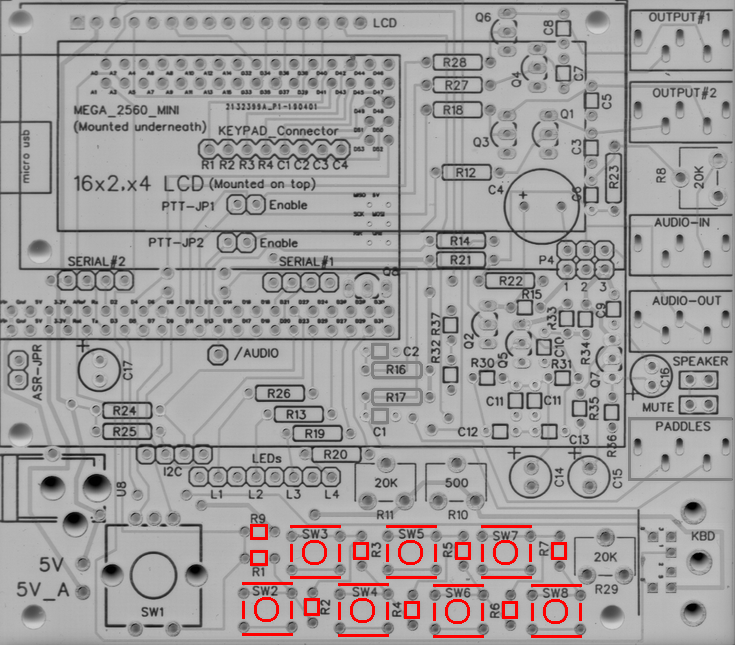
\includegraphics[width=.9\linewidth]{../png/3.2/pcb-top-memory-buttons.png}
\end{center}
\end{itemize}

\newpage
\begin{itemize}
\item[{$\square$}] Rotary Encoder
\begin{itemize}
\item[{$\square$}] SW1 - Rotary encoder with integrated push button
\end{itemize}

This encoder is used to adjust speed, and activate command mode (Button "1").  Depending on enclosure, you may wish to off-board this depending on mounting.  Left to right, the pinouts are:  Counter-Clockwise, Ground, Clockwise.  These are configured using \emph{"FEATURE\_ROTARY\_ENCODER"} in \emph{"keyer\_pin\_settings\_k5bcq.h".}  It is enabled by \emph{"\#define FEATURE\_ROTARY\_ENCODER"} in \emph{"keyer\_features\_and\_options\_k5bcq.h".}
\end{itemize}
\begin{center}
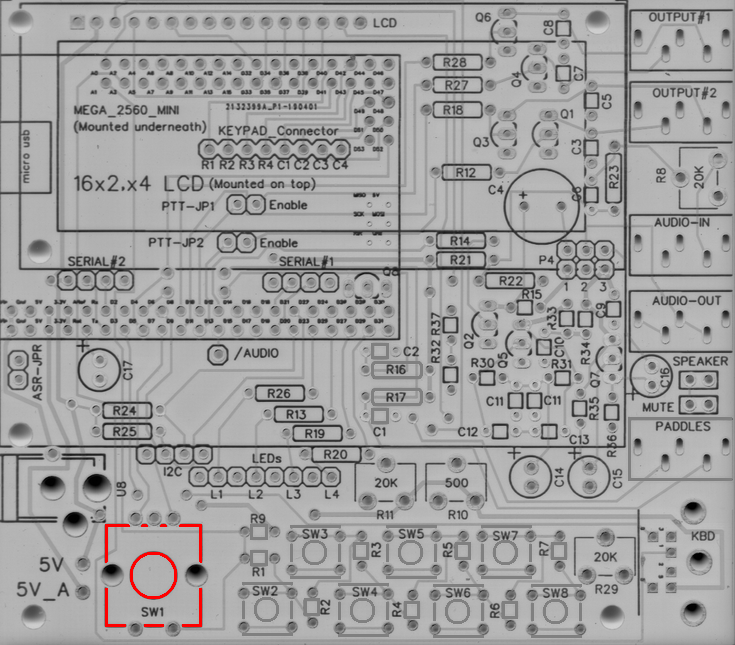
\includegraphics[width=.9\linewidth]{../png/3.2/pcb-top-rotary-encoder.png}
\end{center}

\newpage
\begin{itemize}
\item[{$\square$}] Keyboard Input
\begin{itemize}
\item[{$\square$}] X1 - MINI DIN 6
\end{itemize}

 Keyboard input is enabled using a standard PS/2 keyboard MINI DIN 6 plug.  No additional parts are required.  A PS/2 keyboard is enabled using \emph{"\#define FEATURE\_PS2\_KEYBOARD"} in \emph{"keyer\_features\_and\_options\_k5bcq.h".}  The library used for the keyboard is \emph{"K3NG\_PS2KEYBOARD"} which is included in the provided libraries.  And yes, the library is uncategorized and will trigger a "warning" on compilation - you can safely ignore it.
\begin{center}
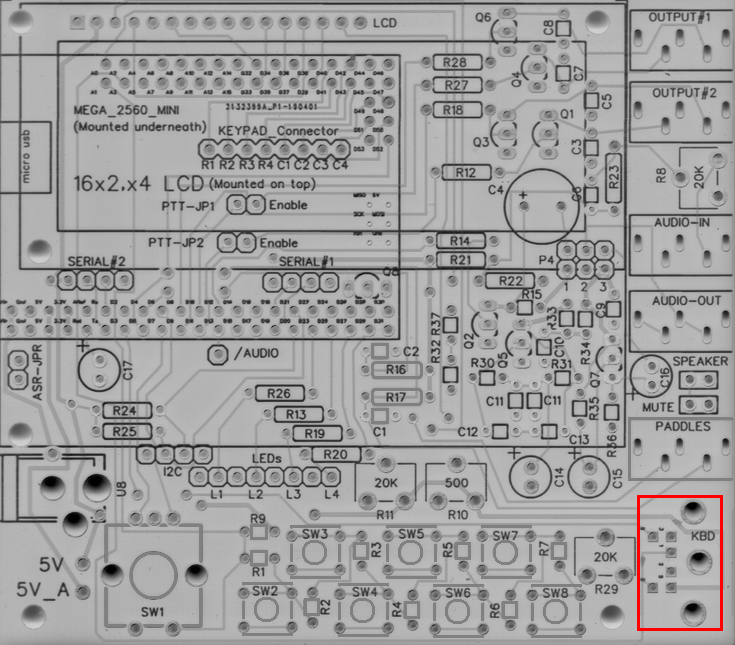
\includegraphics[width=.9\linewidth]{../png/3.2/pcb-top-mini-din-6.png}
\end{center}
\end{itemize}

\newpage
\begin{itemize}
\item[{$\square$}] Keypad
\begin{itemize}
\item[{$\square$}] U3 - 3x4 or 4x4 keypad
\end{itemize}

No additional parts are needed, other than the keypad.  It is likely that you will off-board the connection to the keypad, and thus it is likely that you will prefer to use a 1x8 2.54mm male header for connections, though direct wiring can be done if you so choose.

To enable the use of the keypad, you \textbf{MUST} enable the appropriate module \emph{"\#define FEATURE\_4x4KEYPAD"} or \emph{"\#define FEATURE\_3x4\_KEYPAD"} in \emph{"keyer\_features\_and\_options\_k5bcq.h".}  The pinouts should be correct (matching the PCB markings), but no confirmation has been made at this time.  The pins are set under \emph{"FEATURE\_4x4\_KEYPAD"} and \emph{"FEATURE\_3x4\_KEYPAD"} in \emph{"keyer\_pin\_settings\_k5bcq.h".}
\end{itemize}
\begin{center}
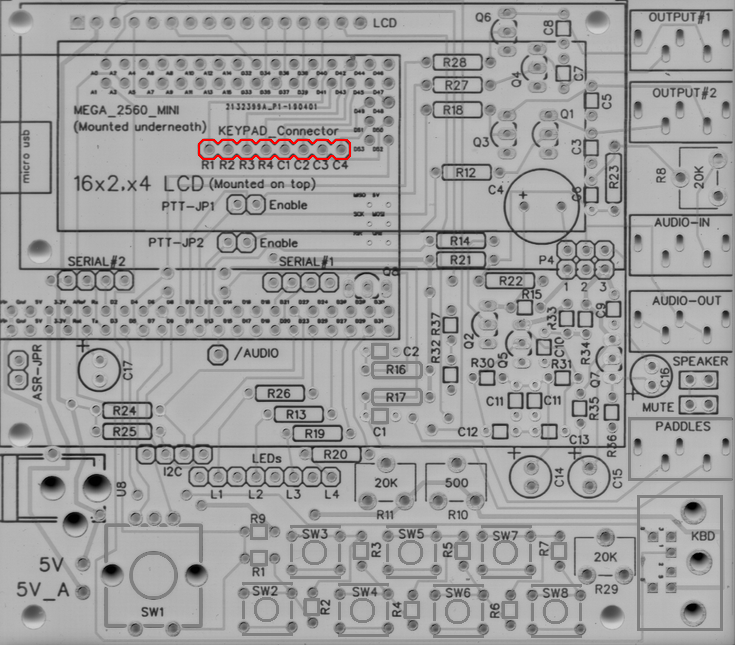
\includegraphics[width=.9\linewidth]{../png/3.2/pcb-top-3x4-keypad.png}
\end{center}
\begin{center}
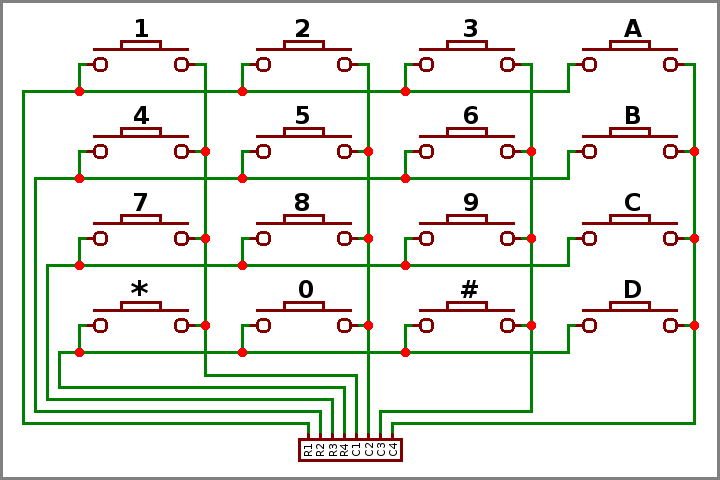
\includegraphics[width=.9\linewidth]{../png/3.2/keypad_layout.png}
\end{center}

\newpage
\begin{itemize}
\item[{$\square$}] Goertzel Audio Decoder
\begin{itemize}
\item[{$\square$}] R8 - 20k\(\Omega\) Trimpot - (203)
\item[{$\square$}] R21, 22 - 10k\(\Omega\) - (Brown-Black-Orange)
\item[{$\square$}] R23 - 100\(\Omega\) - (Brown-Black-Brown)
\item[{$\square$}] C6 - 100nF - (104)
\item[{$\square$}] J3 - 3.5mm TRS Jack
\end{itemize}

Audio input that is decoded using Goertzel algorithm.  R8 is used to help set the audio voltage, and R11 and 22 bias the input voltage +/- 2.5volts.

Information regarding the Goertzel circuit and code used in the K3NG keyer can be found \href{http://skovholm.com/cwdecoder}{here}.  The variables for the Goertzel decoding must be set at compile time, and are \uline{NOT} part of the sketch.  If you wish to edit them, do so in \emph{:goertzel.h:} in the K3NG libraries.  The values for tweaking are \emph{"GOERTZ\_SAMPLES"} and \emph{"GOERTZ\_TARGET\_FREQ".}  Editing these values is a trade off between precision and processing power.  Please consult with the library for more details.
\end{itemize}
\begin{center}
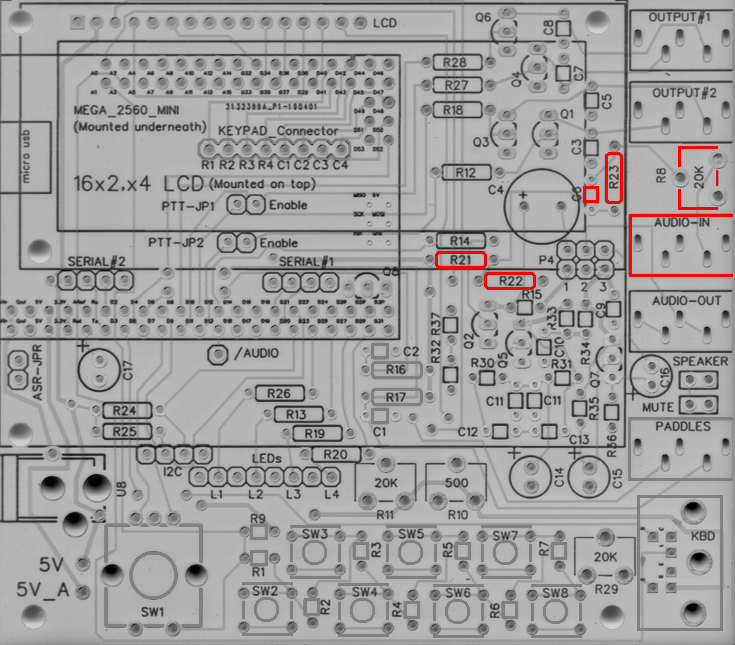
\includegraphics[width=.9\linewidth]{../png/3.2/pcb-top-goertzel-filter.png}
\end{center}

\newpage
\subsection{Outputs}
\label{sec:orgc9d7519}
\begin{itemize}
\item[{$\square$}] Keyer Output 1
\begin{itemize}
\item[{$\square$}] R27, 28 - 1k\(\Omega\) - (Brown-Black-Red)
\item[{$\square$}] C7, 8 - 10nF (103)
\item[{$\square$}] Q4, Q6 - 2N7000 -
\item[{$\square$}] JP1 - 1x2 2.54mm header with jumper
\item[{$\square$}] JX - 3.5mm TRS audio jack
\end{itemize}

Keyer output with PTT.  If you do not wish to be able to enable / disable PTT, you can permanently jumper JP1 with bus wire, a scrap resistor lead, or similar.  Transmit key lines, and PTT line are configured by \emph{"\#define tx\_key\_line\_1"} and \emph{"\#define ptt\_tx\_1"} respectively, in \emph{"keyer\_pin\_settings\_k5bcq.h".}
\end{itemize}
\begin{center}
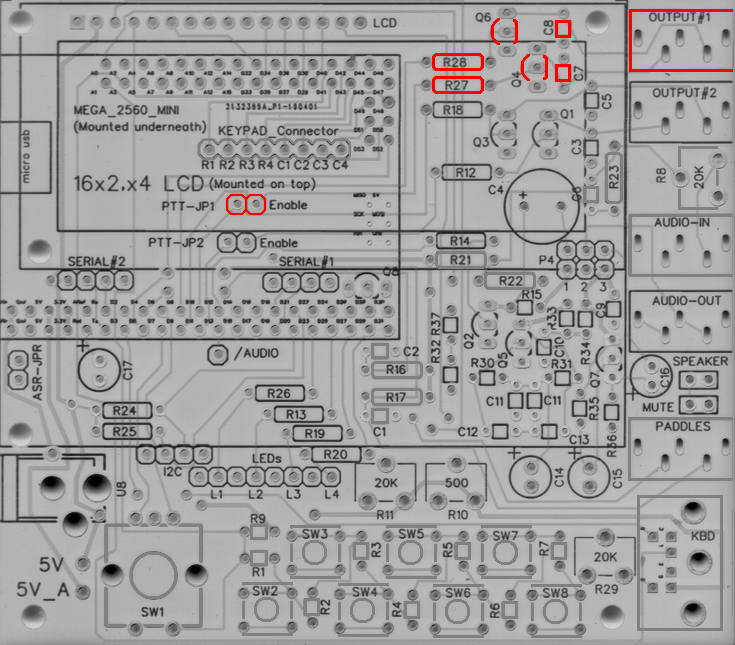
\includegraphics[width=.9\linewidth]{../png/3.3/pcb-top-keyer-output-1.png}
\end{center}

\newpage
\begin{itemize}
\item[{$\square$}] Keyer Output 2
\begin{itemize}
\item[{$\square$}] R12, 18 - 1k\(\Omega\) - (Brown-Black-Red)
\item[{$\square$}] C3, 5 - 10nF (103)
\item[{$\square$}] Q1, Q3 - 2N7000 -
\item[{$\square$}] JP2 - 1x2 2.54mm header with jumper
\item[{$\square$}] JX - 3.5mm TRS audio jack
\end{itemize}

Keyer output with PTT.  If you do not wish to be able to enable / disable PTT, you can permanently jumper JP2 with bus wire, a scrap resistor lead, or similar.  Transmit key lines, and PTT line are configured by \emph{"\#define tx\_key\_line\_2"} and \emph{"\#define ptt\_tx\_2"} respectively, in \emph{"keyer\_pin\_settings\_k5bcq.h".}
\end{itemize}
\begin{center}
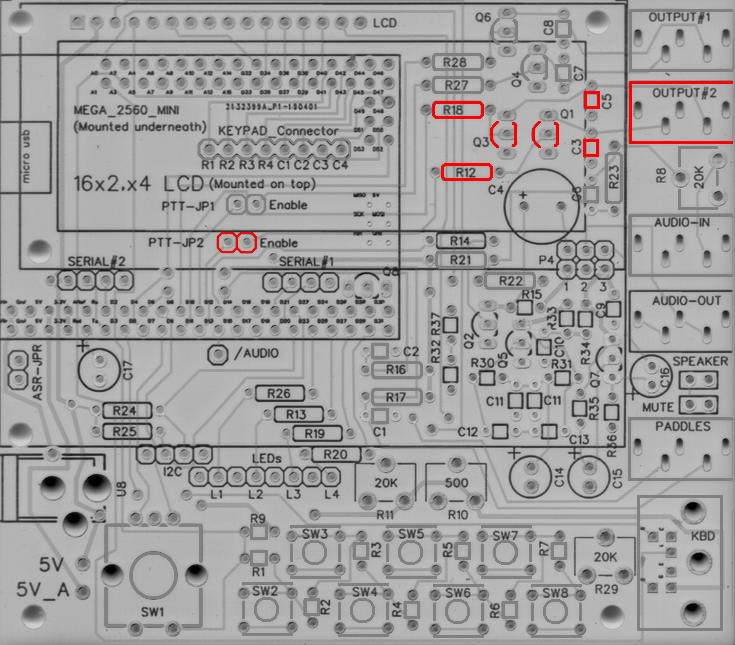
\includegraphics[width=.9\linewidth]{../png/3.3/pcb-top-keyer-output-2.png}
\end{center}

\newpage
\begin{itemize}
\item[{$\square$}] Audio Output
\begin{itemize}
\item[{$\square$}] P4A, P4B - 2, 1x3 or 1, 2x3 2.54mm headers with jumpers
\item[{$\square$}] JX - 3.5mm TRS audio jack
\end{itemize}

This jumper block must be installed if EITHER audio module is to be included.  This allows you to select between the Twin T Oscillator circuit, and the arudino's integrated Square wave output.  You may choose to permanently jumper this if you do not wish to be able to switch.  If you wish to use the TWIN T oscillator, install those parts, and place the jumpers on pins 2 \& 3 of the headers (right 2), for both P4A and P4B.  If you wish to use the square wave output, install those parts, and place the jumpers on pins 1 \& 2 of the headers (left 2), for both P4A and P4B.

The audio is sent out to JX from both audio modules - no configuration changes are required, no matter which audio option you select.

The sketch defaults to the much more pleasant sounding, 600Hz Twin T oscillator.  No configuration changes are necessary.  To enable the Pulse-Width-Modulation square wave output, you must comment out \emph{"\#define OPTION\_SIDETONE\_DIGITAL\_OUTPUT\_NO\_SQUARE\_WAVE"} in \emph{"keyer\_features\_and\_options.h"} (it causes high/low logic instead of the PWM).  After doing so, you \textbf{must} \uline{also} change the pin sending the audio from 31, to 12.  This is found under \emph{"\#define sidetone\_line"} in \emph{"keyer\_pin\_settings\_k5bcq.h".}

The sidetone can be toggled between "On", "Paddles Only", and "Off" using \texttt{"O"} in command mode (and \texttt{\textbackslash{}O} in the command line interface).  This setting is stored between powerdowns.  It functions with both Twin T and Square wave output.
\end{itemize}
\begin{center}
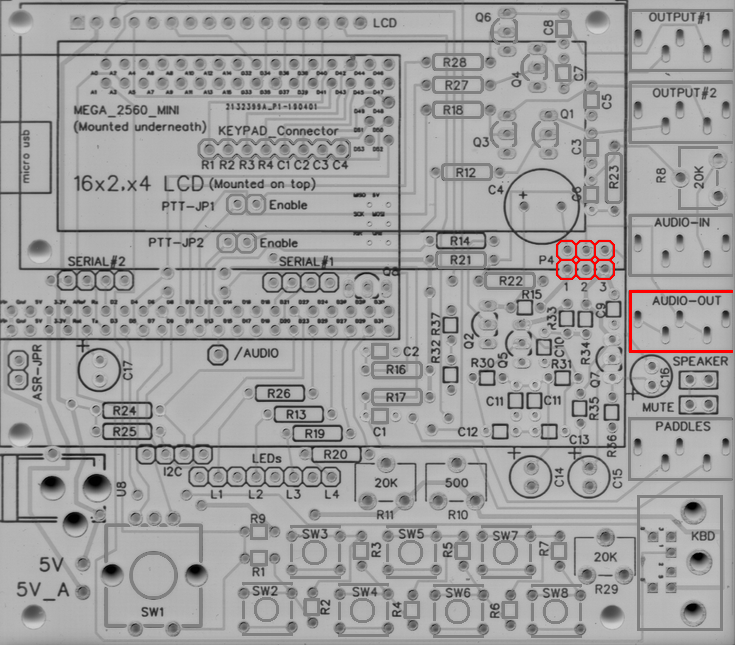
\includegraphics[width=.9\linewidth]{../png/3.3/pcb-top-audio-output.png}
\end{center}

\newpage
\begin{itemize}
\item[{$\square$}] Audio Output (Twin T Oscillator)
\begin{itemize}
\item[{$\square$}] R29 - 20k\(\Omega\) trimpot - (204)
\item[{$\square$}] R30, 31, 33 - 3.3k\(\Omega\) - (Orange-Orange-Red)
\item[{$\square$}] R32 - 560\(\Omega\) - (Green-Blue-Brown)
\item[{$\square$}] R34 - 10\(\Omega\) - (Brown-Black-Black)
\item[{$\square$}] R35 - 150k\(\Omega\) - (Brown-Green-Yellow)
\item[{$\square$}] R36 - 100\(\Omega\) - (Brown-Black-Brown)
\item[{$\square$}] R37 - 100k\(\Omega\) - (Brown-Black-Yellow)
\item[{$\square$}] C9, 10, 11a, 11b, 12, 13 - 100nF - (104)
\item[{$\square$}] C14, 15, 16 - 10uF Electrolytic
\item[{$\square$}] Q5, 7 - 2N3904
\item[{$\square$}] Q8 - 2N7000
\end{itemize}

The audio output of this circuit generates a pure sine wave at a hardware-defined frequency, determined by the values of the components in the circuit, and these values have been configured for 600Hz.  These values can be readily modified to change the desired frequency - but that is beyond the scope of this document.  The circuit uses the high/low logic from Pin 31, and inverts it with Q8.  The advantage is the audio quality - the disadvantage of this circuit is the inability to modify the sidetone without replacing the parts.
\end{itemize}
\begin{center}
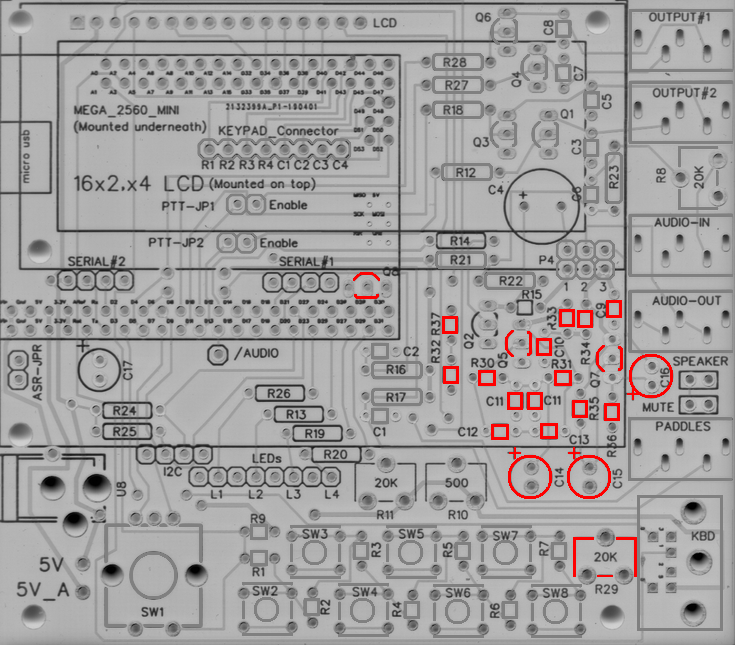
\includegraphics[width=.9\linewidth]{../png/3.3/pcb-top-audio-output-twin-t.png}
\end{center}

\newpage
\begin{itemize}
\item[{$\square$}] Audio Output (Square Wave)
\begin{itemize}
\item[{$\square$}] R14 - 100\(\Omega\) - (Brown-Black-Brown)
\item[{$\square$}] R15 - 220\(\Omega\) - (Red-Red-Brown)
\item[{$\square$}] C4 - 100uF - Electrolytic
\item[{$\square$}] Q2 - 2N3904
\item[{$\square$}] JX - 3.5mm TRS audio jack
\end{itemize}

The audio output using the Square Wave output is a tone generated by Pulse-Width Modulation.  While not nearly as nice sounding as the Twin T, it has a number of advantages.  Its tone can be adjusted using \texttt{"F"} in the command mode (and \texttt{\textbackslash{}f \#\#\#} in the command line interface), to the users preference at any time.  The setting is saved between powerdowns.  The default value (i.e. first boot and factory reset) is set by \emph{"\#define initial\_sidetone\_freq"} in \emph{"keyer\_settings\_k5bcq.h".}  The limits (low and high) are set by \emph{"\#define sidetone\_hz\_limit\_low"} and \emph{"\#define sidetone\_hz\_limit\_high"} respectively, in the same file.
\end{itemize}
\begin{center}
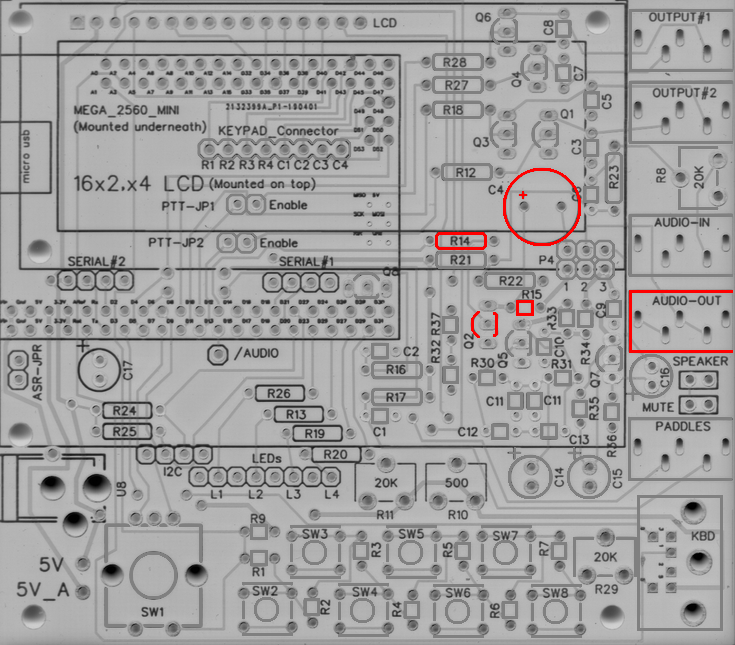
\includegraphics[width=.9\linewidth]{../png/3.3/pcb-top-audio-output-square-wave.png}
\end{center}

\newpage
\begin{itemize}
\item[{$\square$}] Speaker Output
\begin{itemize}
\item[{$\square$}] SP1 - Speaker
\item[{$\square$}] P2 - 1x2 2.54mm male header
\end{itemize}

SP1 is hookups for an optional, off-board speaker.  Audio output is taken from both Twin T and Square Wave outputs, so no modification is necessary.  The circuit is designed to mute if Audio Output plug is in use.  P2 is an optional jumper, that allows you to detach the speaker from ground, muting the speaker output. (jumpered = on, unjumpered = muted)
\end{itemize}
\begin{center}
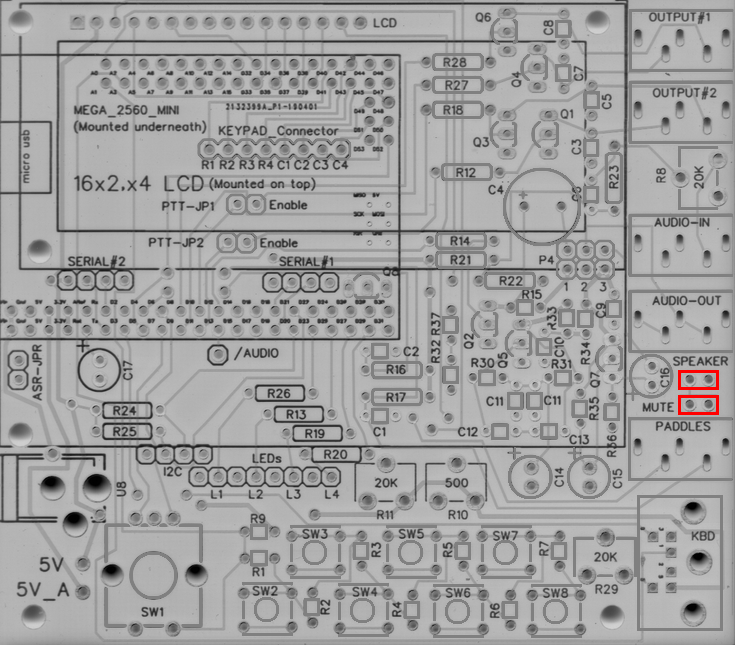
\includegraphics[width=.9\linewidth]{../png/3.3/pcb-top-speaker-output.png}
\end{center}

\newpage
\subsection{Displays / Indicators}
\label{sec:org5d5f8b0}
There are number of inexpensive LCD displays that are available from a number of sources.  There are too many to list individually, but suffice it to say, if it uses serial or i2c, you can hook it up.

There are multiple settings for displays.  The assigned pins are set by \emph{"defined(FEATURE\_LCD\_4BIT)"} in \emph{"keyer\_pin\_settings\_k5bcq.h"} for serial displays.  i2c is configured by enabling the appropriate i2c option in \emph{"keyer\_features\_and\_options.h",} based on the hardware you are using.  The k5bcq configuration comes defaulted to a serial, 1602 display.  To adjust the LCD display size (serial or i2c - 1604, 2004, etc), change \emph{"define LCD\_COLUMNS"} and \emph{"define LCD\_ROWS"} to their appropriate values in \emph{"keyer\_settings\_k5bcq.h".} 

\begin{itemize}
\item[{$\square$}] LCD Display (Serial)
\begin{itemize}
\item[{$\square$}] R10 - 500\(\Omega\) - 6mm top-adjust trimpot
\item[{$\square$}] R11 - 20k\(\Omega\) - 6mm top-adjust trimpot
\item[{$\square$}] U1 - LCD display (1602, 1604, 2004)
\item[{$\square$}] 1x16 2.54mm male \& female headers

Description of the installation of a display is relatively \emph{difficult.}  Not because the process is difficult, but due to the variety.  Suffice it to say, the description is much more difficult than the execution.  To install a serial display (1602, 1604, 2004), connect them via the 16 pin "LCD" headers.  To install attached to the board, use the same process as the installation of the Arduino - cut appropriate lengths (1x16) male and female headers, and lightly combine the headers.  Sandwich them between the display and the PCB, and solder the ends.  Once you've made sure they're flush and perpendicular with their respective boards, finish soldering the pins.  Install R10 and R11 to control the display's backlight and contrast, respectively.

\emph{Builders note:  Installing spacers on the display and using them to ensure level installation is highly recommended.  It makes the entire job easier, and results in a neater product - even if you have no intention of leaving them in place.  Mounting holes have been added to the board to affix the display if you so choose.  (Also recommended)}
\end{itemize}

\emph{Builders note:  Adjust the backlight to the desired level first, then adjust contrast until just after the blocks disappear on the display.  This will provide the crispest looking display.}
\end{itemize}
\begin{center}
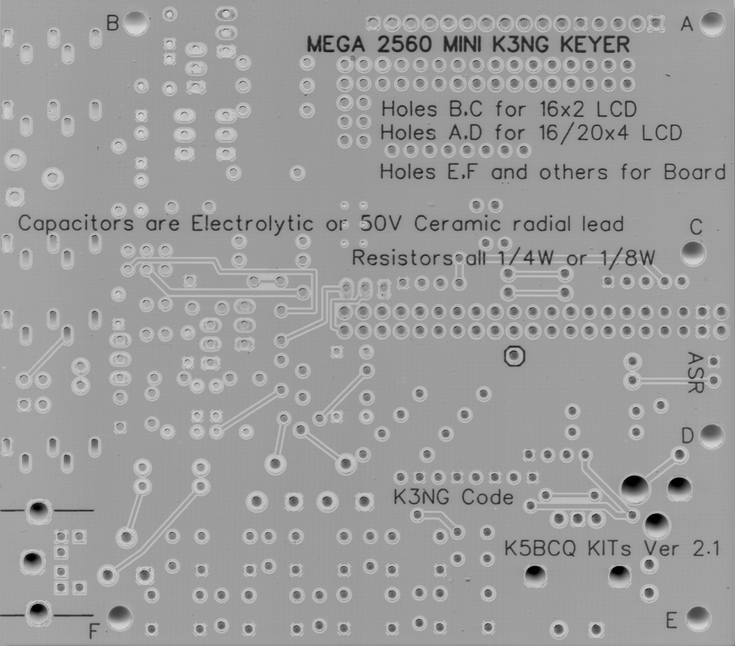
\includegraphics[width=.9\linewidth]{../png/3.4/pcb-bot-display-serial.png}
\end{center}
\begin{center}
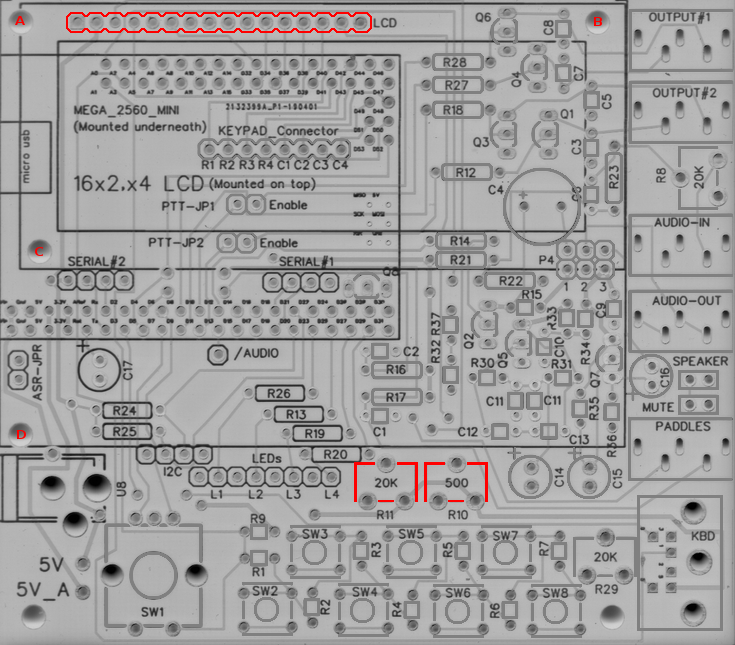
\includegraphics[width=.9\linewidth]{../png/3.4/pcb-top-display-serial.png}
\end{center}

\newpage
\begin{itemize}
\item[{$\square$}] I2C Display
\begin{itemize}
\item[{$\square$}] U1 - LCD display (1602, 1604, 2004)
\item[{$\square$}] 1x4 2.54mm male \& female headers
\item[{$\square$}] Dupont wires or similar

The installation of an i2c display is similar to that of a standard serial display, but is complicated by the location of the i2c headers and device pinouts.  You will likely need to off-board the i2c display.  Individual configurations are beyond the scope of this document, but suffice to say - install headers and/or jumper wires and connect as labeled.

\emph{Builders note:  Left to right, the i2c pins are:  +5volts, SDA, SCL, Ground.  You may also need to adjust the i2c device address in the main keyer file (k3ng\_keyer.ino), if you are having difficulty connecting using some of the i2c hardware.  This is rare, but possible - particularly when using inexpensive Chinese clones.}
\end{itemize}
\end{itemize}
\begin{center}
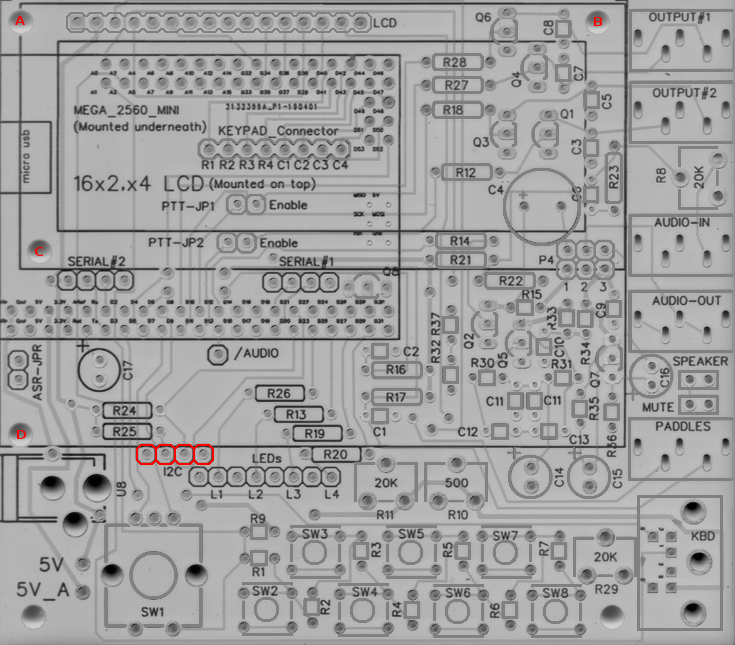
\includegraphics[width=.9\linewidth]{../png/3.4/pcb-top-i2c-display.png}
\end{center}
\begin{center}
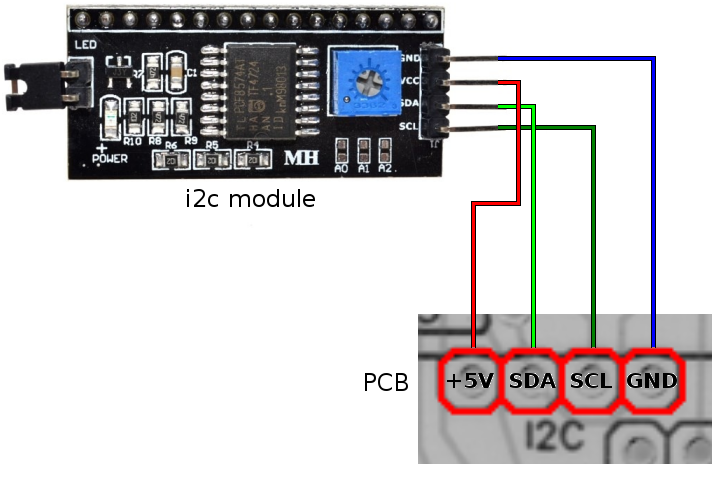
\includegraphics[width=.9\linewidth]{../png/3.4/i2c_1602LCD.png}
\end{center}
\newpage
\begin{itemize}
\item[{$\square$}] LED Indicators
\begin{itemize}
\item[{$\square$}] R13, 19, 20, 26 - 220\(\Omega\) - (Red-Red-Brown)
\item[{$\square$}] LED1, 2, 3, 4 - LEDs of your color choice
\end{itemize}

LED indicators for command mode, audio input for Goertzel decoder, and Right / Wrong for sending practice.  These can easily be modified for different purposes, if you like.  Depending on your enclosure design, you may wish to add headers instead of the LEDs themselves, so you can readily off-board them to elsewhere on your enclosure.  See \emph{"keyer\_pin\_settings\_k5bcq.h"} for changing pin assignments.  The sketch's default settings are:

\begin{center}
\begin{tabular}{lrl}
LED & Pin & Default Setting\\
\hline
LED 1 & 23 & CW Decoder Indicator\\
LED 2 & 25 & Send Practice Wrong\\
LED 3 & 27 & Send Practice Correct\\
LED 4 & 29 & Command Mode Indicator\\
\end{tabular}
\end{center}
\end{itemize}
\begin{center}
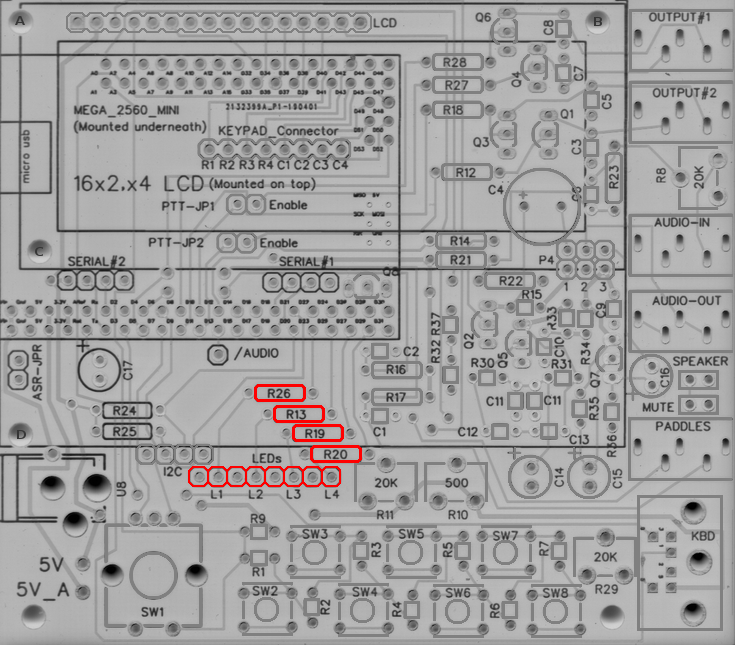
\includegraphics[width=.9\linewidth]{../png/3.4/pcb-top-led-indicators.png}
\end{center}

\newpage
\subsection{Miscellaneous}
\label{sec:orgd6581ad}
\begin{itemize}
\item[{$\square$}] DC Power Jack
\begin{itemize}
\item[{$\square$}] J6 - 2.1x5.5mm DC Barrel Socket

This is DC input of 7-12v.  It is routed to the Voltage In lines on the Arduino, and takes advantage of its linear voltage regulator to output 5v to all of the other parts.  Note:  a battery or other voltage in can readily be installed using the Pad just above the socket's ground.
\end{itemize}
\end{itemize}
\begin{center}
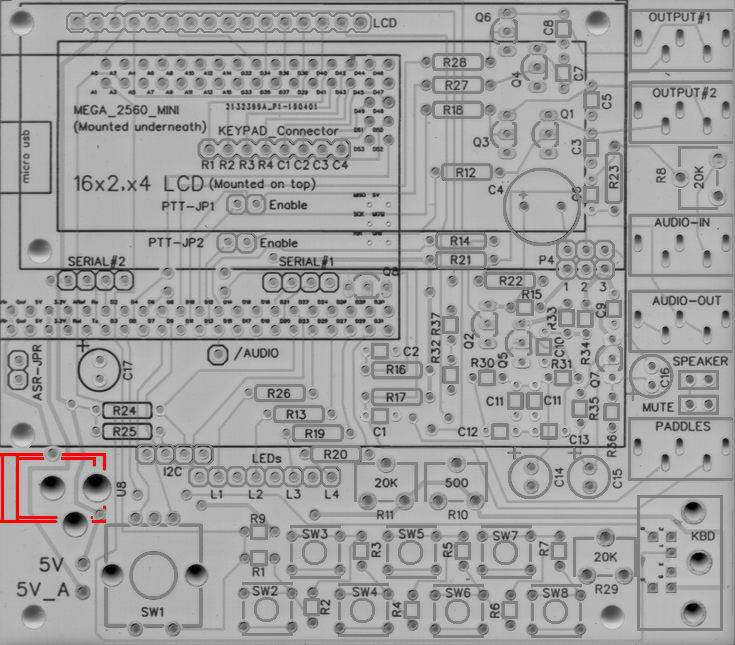
\includegraphics[width=.9\linewidth]{../png/3.5/pcb-top-dc-power-jack.png}
\end{center}

\newpage
\begin{itemize}
\item[{$\square$}] ASR Jumper, PTT Jumper TX\_1, PTT Jumper TX\_2
\begin{itemize}
\item[{$\square$}] 1x2 - 2.54mm male header and jumper (each option)

You can adjust these features by jumpering these connections with bus wire or scrap resistor leads.  However, it's likely a better idea to install 1x2 2.54mm headers and jumpers.  This allows you the ability to enable / disable them quickly and easily.
\end{itemize}
\end{itemize}
\begin{center}
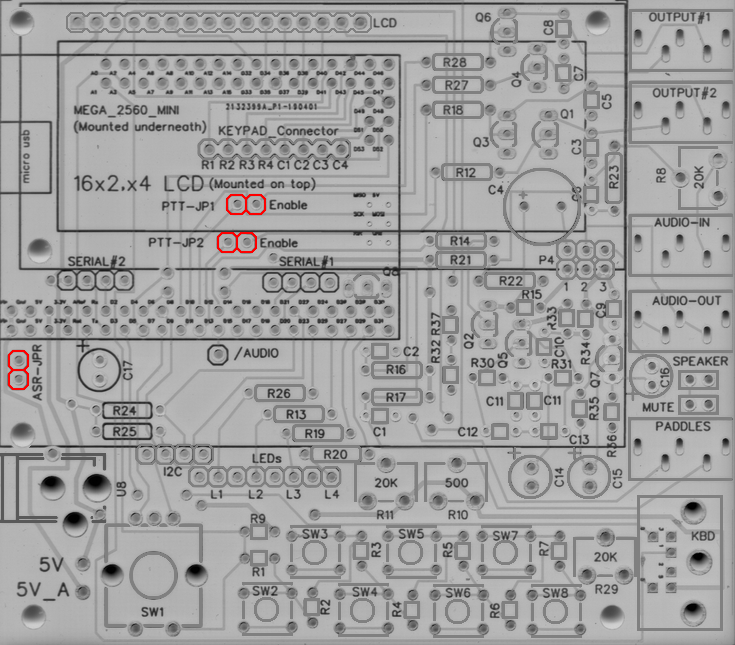
\includegraphics[width=.9\linewidth]{../png/3.5/pcb-top-asr-ptt1-ptt2-jumpers.png}
\end{center}

\newpage
\begin{itemize}
\item[{$\square$}] Power Jumper

\begin{itemize}
\item This set of pads allows you to either power the peripherals using the 5 volt output of the arduino, or input 5v from an external source to power them.  If you plan to use it independent of a computer, you likely will just permanently jumper this.
\end{itemize}
\end{itemize}
\begin{center}
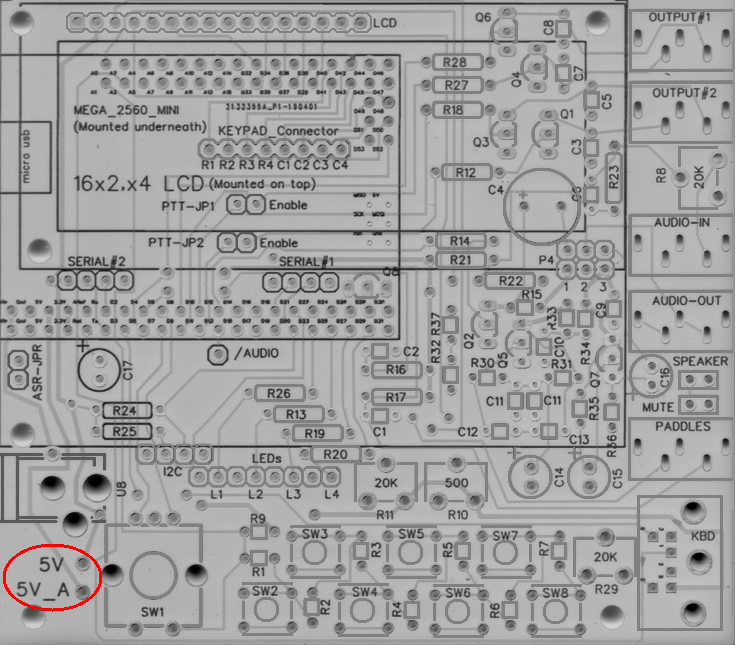
\includegraphics[width=.9\linewidth]{../png/3.5/pcb-top-power-jumper.png}
\end{center}

\newpage
\section{Flashing Instructions}
\label{sec:orgd927fdd}
The code for the K3NG keyer, in any of its designs (homebrew or otherwise!) resides on the \href{https://github.com/k3ng/k3ng\_cw\_keyer}{K3NG Github}.  Goody has kindly including pull requests to enable hardware for this build into the K3NG main code, resulting in a very easy method for flashing the most recent code and features!

\begin{enumerate}
\item Download the code from \href{https://github.com/k3ng/k3ng\_cw\_keyer}{K3NG Github}.
\item Unpack (unzip) the arduino project wherever you like.  The convention is in the \$HOMEDIR\Arduino folder.
\begin{itemize}
\item \emph{If you git cloned the repo\ldots{} you likely don't need me to explain the rest of this process to you\ldots{}}
\end{itemize}
\item Make sure you have the code (containing the k3ng\_keyer.ino and a bunch of .h files) in a folder name k3ng\_keyer.  If you do not, the Arduino IDE will complain, and likely move the file on you.
\item Copy the contents of the library folder (k3ng\_cw\_keyer/libraries) to your Arduino/libraries folder ("\textasciitilde{}/Arduino/libraries" on Linux).
\begin{itemize}
\item \emph{Depending on your method and location of extraction, you may just skip this step.}
\end{itemize}
\item Open the Sketch.  The actual sketch file is \emph{"k3ng\_keyer.ino".}
\begin{itemize}
\item You can open it either by double-clicking on the file in your file explorer, or \emph{"File \(\rightarrow\) Open"} in the Arduino IDE.
\end{itemize}
\item Your path now splits.  You can either:
\begin{itemize}
\item Edit the keyer configuration files by hand to enable every feature you want, and assign the pins yourself (in which case you'll edit \emph{"keyer\_features\_and\_options.h", "keyer\_pin\_settings.h", "keyer\_settings.h",} and possibly \emph{"keyer\_debug.h".}
\item Enable a hardware configuration by un-commenting (deleting the \texttt{//} from the front of a line) a single line - \emph{"\#define HARDWARE\_K5BCQ"} from \emph{"keyer\_hardware.h".}
\end{itemize}
\item Since we're going to assume you chose the second option, you \emph{should} be good to go.  This configuration has all of the pin settings already performed, and all non-invasive options turned on.  If you want to enable or disable anything, now is the time.  Features can be enabled by uncommenting them in \emph{"keyer\_features\_and\_options\_k5bcq.h"}, and can be disabled by commenting them back out.  Pin settings can be adjusted as well.  be sure to edit them as described in the code (and in the above build section).
\begin{itemize}
\item \textbf{REMEMBER} this configuration comes with the Twin T oscillator as default.  If you are using the square wave output, please adjust the values noted in the code (and documented in the build section).
\end{itemize}
\item Connect the Arduino to your computer using the USB cable.
\begin{itemize}
\item If this is done with the Arduino connected to the PCB, be sure to \textbf{remove} (unjumper) the ASR jumper.  It won't work for you if you don't.  Reinstall when you're done.
\end{itemize}
\item Set up your board in the Arduino IDE.
\begin{itemize}
\item The Arduino Mega 2560 Pro Mini has the same pinouts, chip, and specs as the full-size Mega.  Thus, no additional boards need to be installed.  To select it:  Tools \(\rightarrow\) Board \(\rightarrow\) Arduino AVR Boards \(\rightarrow\) "Arduino/Genuino Mega or Mega2560"
\item You shouldn't need to adjust it, but make sure that the correct processor is selected.  To check:  Tools \(\rightarrow\) Processor \(\rightarrow\) "ATmega2560 (Mega2560)"
\item Select the appropriate port.  You likely will only have one available.  To select it:  Tools \(\rightarrow\) Port \(\rightarrow\) Whichever is available
\item You shouldn't need to adjust it, but make sure you have the correct programmer selected.  To check:  Tools \(\rightarrow\) Programmer \(\rightarrow\) "AVRISP mkII".  Others will likely work, but this default has always worked for me.
\end{itemize}
\item Click "Upload"
\begin{itemize}
\item This will automatically compile the code, save it, and transmit it to the attached Arduino
\item You can safely ignore the error regarding the "K3NG\_PSKeyboard" library being the wrong category.  It's just a warning.
\end{itemize}
\item Wait patiently.  The message window at the bottom will keep you updated on how it's progressing (compile, upload, errors).  When it indicates that the upload is finished, you can disconnect the Arduino, and your keyer is ready to go!
\end{enumerate}

\newpage
\section{Schematic}
\label{sec:org4a9493b}
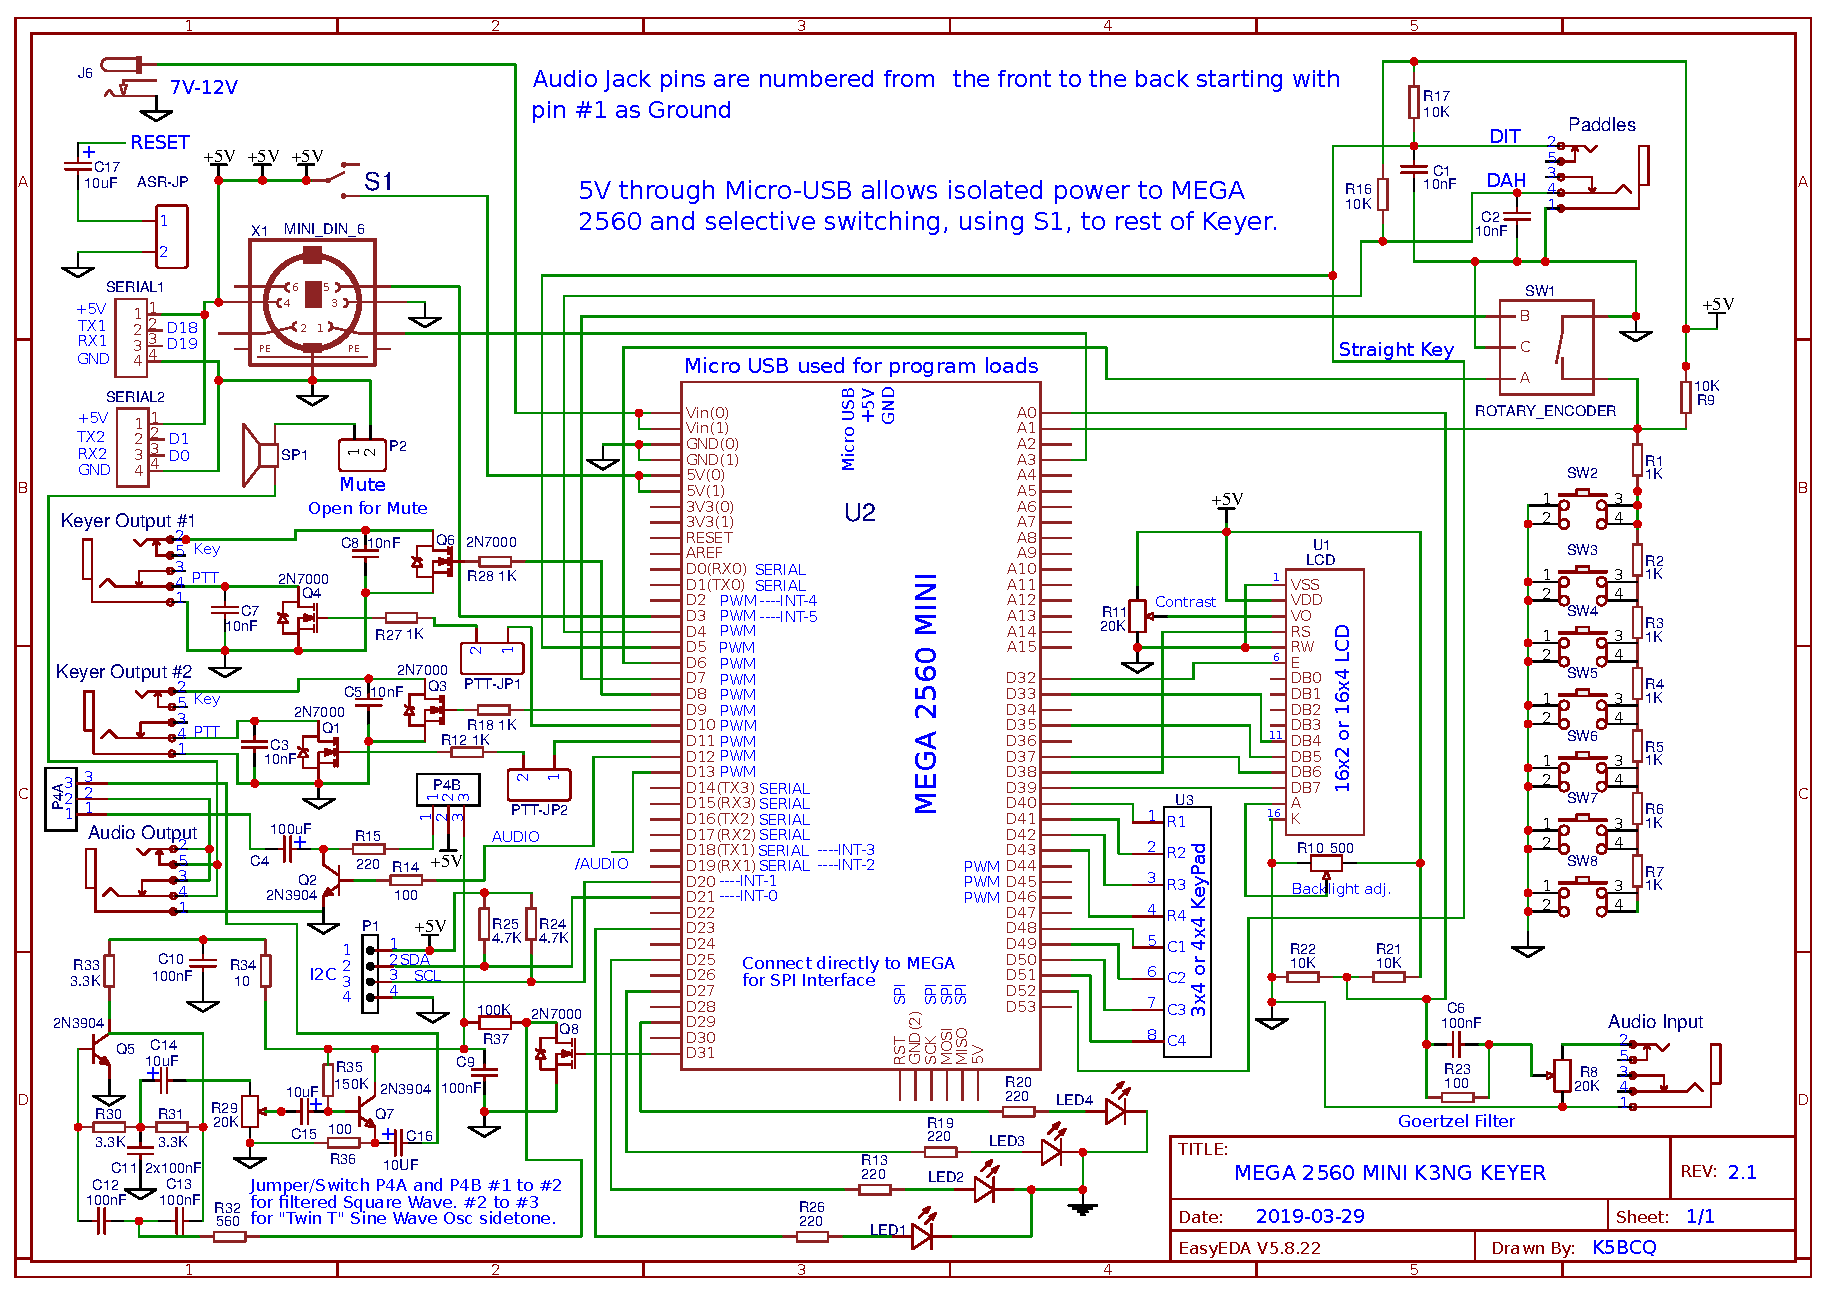
\includepdf[angle=90]{../Schematic_BIG-Keyer_Sheet-1_20190329121109.pdf}
\end{document}